\chapter{Fluorescence time-lapse imaging of the NER process}
\label{chap:quantData}
\pagestyle{plain}


Mon\'{e} and colleagues (2001) advanced the research on nucleotide excision repair (NER) essentially by developing a technique to UV-irradiate a cell's nucleus within a locally confined area \cite{Mone2001}. Until then, the \textit{in-vivo} analysis of NER was limited to measurements of enzyme mobility and exchange dynamics at steady state performed with photobleaching experiments after irradiation of the whole nucleus \cite{Houtsmuller2001,Mone2004,Vermeulen2011}. In contrast, the enclosed amount of single-stranded DNA damages causes the local activation of a multi-protein repair machinery, which in turn allows us to study the \textit{de-novo} assembly and dissociation kinetics of individual repair factors. Exploiting this standard experimental set-up, Luijsterburg \text{et.\ al.} collected a comprehensive time-series dataset comprising the accumulation and dissociation of seven individual repair enzymes.\\ 
In the following chapter we will introduce this data together with the experimental methods, which represent the basis for our quantitative analysis of the NER process. We were able to augment the measurements with a direct readout for newly-synthesized DNA following the incorporation of the fluorescently modified nucleotide analogue EdU. It turns out that the DNA repair process is essentially a slow first-order reaction with a half-life of 1.2 hours.   \\


The experiments reported in this chapter were planed and conducted by Martijn Luijsterburg (accumulation and FLIP experiments; Leiden University) and Paul Verbruggen (EdU incorporation; University of Amsterdam).
	
	


\section{Locally UV-inflicted DNA damage}
\label{sec:local_irradiation}
 

To observe the dynamic behaviour of NER factors upon local infliction of DNA damage, we applied the experimental set-up developed by Mon\'e \textit{et al.} (2001)\cite{Mone2001}, in which NER-competent cells are covered with a polycarbonate UV filter containing pores with a given diameter (cf.\ Figure \ref{fig:accuMethod}A). For our purposes, cells were grown on uncoated 24 mm coverslips before being overlaid with a mask with pores of 5 \textmu m diameter \cite{Verbruggen2014}. Figure \ref{fig:accuMethod}B illustrates the realistic deviation of pore diameters due to manufacturing inaccuracies. The expected size deviation has a very small coefficient of variation (CV) of 0.14 indicating a negligible effect on the filter's transmissivity. Filter-covered cells were immediately irradiated with a dose of 100 $\text{J/m}^\text{2}$ of UV-C with a fluency of 3.85 $\text{W/m}^\text{2}$. Due to the specific pore density (4 x $\text{10}^\text{5}$ pores/$\text{cm}^\text{2}$), we could observe nuclei containing only either one damage spot or no spot at all. Two spots per cell were only observed very rarely (cf.\ Figure \ref{fig:accuMethod}C, white arrows indicate the damage spot). With this technique we were able to measure DNA repair in damaged nuclei as well as undamaged control nuclei in the same experiment.

\begin{figure}[t!]
	\begin{center}
		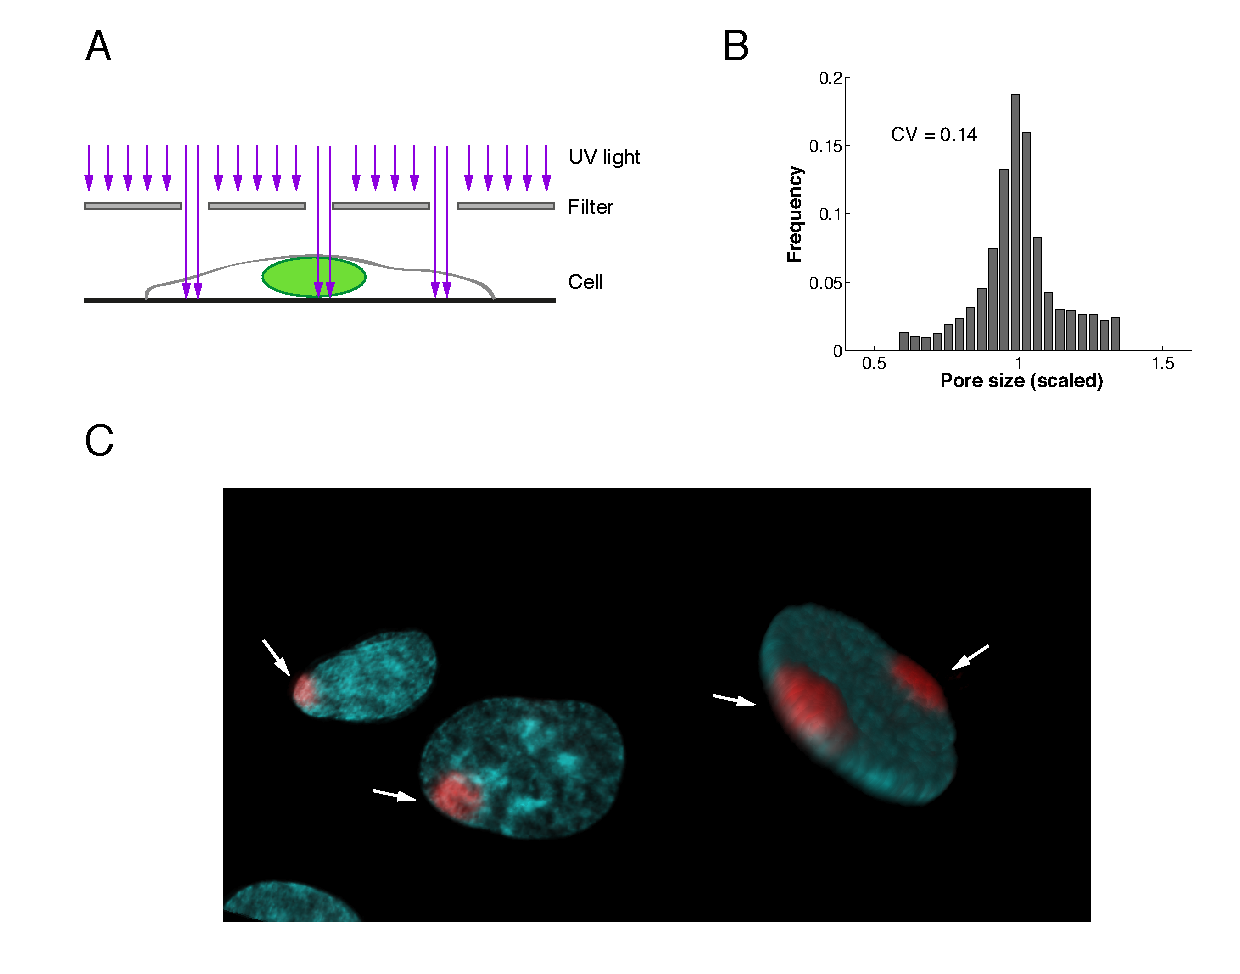
\includegraphics[width=1\textwidth]{Abbildungen/figure2_1.pdf}
		\caption{\textbf{Local irradiation leads to spatially confined DNA damage.} A) Schematic illustration of the experimental set-up. UV-light (purple arrows) is transmitted through a UV filter containing pores with 5 \textmu m diameter. Local irradiation of the chromatin occurs if a pore is located above a cell nucleus. (reprinted Figure from \cite{Terstiege2010}) B) Distribution of the pore sizes within the UV irradiation mask (n=5008) - \textbf{ask paul how he did it} C) Partially UV-irradiated nuclei of cultivated mammalian cells were made visible with a blue-fluorescent DNA stain. Red fluorescence depicts incorporation of labelled nucleotides due to NER.}
		\label{fig:accuMethod}
	\end{center}
\end{figure}

\section{Repair factor accumulation and dissociation occur on different time scales}
\label{subsec:AccuFlipExp}
The ability to locally inflict DNA damage with a discrete dose of UV-C allows for the study of accumulation and exchange behaviour of fluorescently-tagged repair proteins under different experimental conditions. In the following, we describe the comprehensive dataset acquired by Luijsterburg \textit{et al.} (2010)\cite{Luijsterburg2010}, which represents the basis for our quantitative analysis of the NER process. In total, the kinetics of seven repair factors were measured: i) XPC, the lesion recognition factor, ii) TFIIH, the helicase responsible for DNA unwinding, iii) XPA and RPA, which bind and thereby protect single stranded DNA against cleavage, iv) the exonucleases XPF/ERCC1 and XPG performing the incision of the damaged DNA strand and, v) PCNA, which loads the DNA polymerase and hence indirectly provides insight into the DNA repair-synthesis kinetics. \\
Each repair factor were exogenously tagged with a green fluorescent protein (GFP) (or its 'enhanced' derivative EGFP) and expressed at physiological levels within the cell nucleus. Before the cells have been UV-irradiated at time t = 0, the repair proteins were homogeneously distributed at steady state. Immediately afterwards, the repair factors accumulated at the damaged chromatin sites, which led to a higher visible fluorescence intensity (cf.\ Figure \ref{fig:accuImage}A). For quantification of the fluorescence intensity, image analysis was done by using ImageJ software (NIH Bethesda, MD). Accumulated repair-factor concentrations were determined by multiplying the nuclear reference concentrations (cf.\ Table \ref{tab:nuclearconcentrations}) with the fraction of bound proteins at damaged DNA:
% * <l.adlung@dkfz.de> 2014-12-06T23:21:59.631Z:
%
%  expressed at physiological levels under the endogenous promoter?
%
\begin{equation}
Bound \, fraction = (I_\text{LD} - I_\text{outspot})A_\text{LD}/ (I_\text{nucleus} - I_\text{background})A_\text{nucleus}
\label{Eqn:BoundFraction}
\end{equation}     
where $I_\text{LD}$, $I_\text{outspot}$, $I_\text{nucleus}$ and $I_\text{background}$ represent the average fluorescence intensities within the locally damaged spot, an equally sized area in the non-damaged nucleus, the whole nucleus and the background, respectively (cf.\ Figure \ref{fig:accuImage}B). $A_\text{LD}$ and $A_\text{nucleus}$ give the size of the damaged area and the size of the nucleus. Finally, the concentrations of accumulated protein are calculated assuming a damaged nuclear volume of 0.3 pL \cite{Luijsterburg2010}.\\    

 \begin{table}[h!]
 \centering
\begin{tabular}{ccc}
\hline
\textbf{Protein} & \quad \textbf{Concentration} \quad& \quad \textbf{Bound fraction}\\ \hline
XPC\hspace{1cm}&0.140 \textmu M&13\%\\ 
TFIIH&0.360 \textmu M&10\%\\  
XPG&0.440 \textmu M&9\%\\  
XPA&1.110 \textmu M&7\%\\  
\quad XPF/ERCC1 \quad&0.170 \textmu M&7\%\\  
RPA&1.110 \textmu M&15\%\\  
PCNA&1.110 \textmu M&20\%\\  \hline
\end{tabular}
 \caption{\textbf{Nuclear concentrations of NER factors (in \textmu M)} All nuclear quantities are based on published data or on previous estimates \cite{Araujo2001,Houtsmuller1999,Mone2004}. The nuclear concentrations were taken from Luijsterburg \textit{et.\ al.} \cite{Luijsterburg2010} were a nuclear volume of 0.3 pL was assumed. The bound fractions were determined by Eqn.\ \ref{Eqn:BoundFraction}. }\label{tab:nuclearconcentrations}
  \end{table}
% * <l.adlung@dkfz.de> 2014-12-06T23:29:58.578Z:
%
%  Precisely mention irradiation and cell type
%
  
During the timespan of DNA repair, NER factor concentrations rise at the sites of local damage and then gradually decrease from their plateau levels at different rates (cf.\ Figure \ref{fig:accuImage}C). For example, the half-time $t_\text{1/2}$ for XPC- and XPG-EGFP is $\sim$1 h whereas XPA-EGFP has a longer half-time of $\sim$2.5 h \cite{Luijsterburg2010}. In contrast, PCNA and RPA stay present in the damage spot even after lesion removal. These results show that NER factors engage for hours in the repair process with temporal changes in the molecular composition.\\
\begin{figure}[t!]
	\begin{center}
		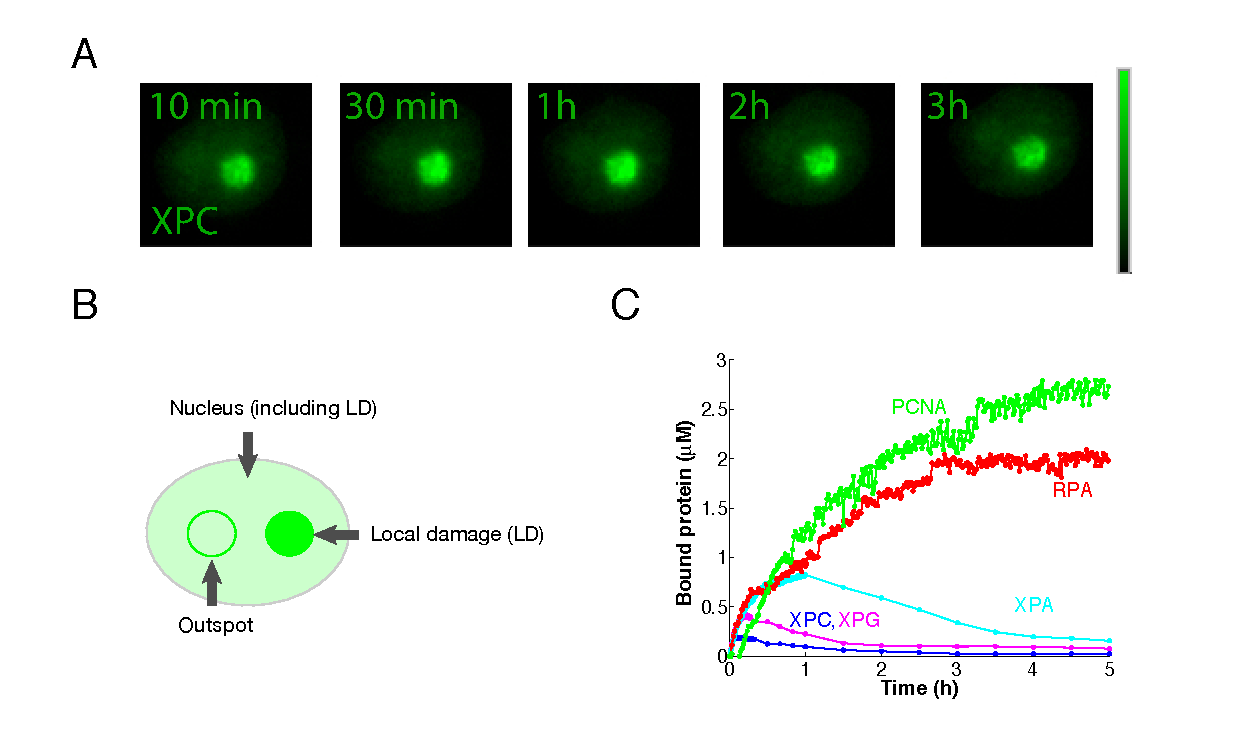
\includegraphics[width=1\textwidth]{Abbildungen/figure2_2.pdf}
		\caption{\textbf{Fluorescently labelled NER factors accumulate at locally irradiated nucleus.} A) XPC-eGFP  stably expressed in XP-C cells  after local irradiation with UV-C (100 J$\text{m}^{-\text{2}}$ through 5-\textmu m-diameter pores). XPC-eGFP accumulates at sites of local DNA damage.  B) Scheme of a locally UV-irradiated nucleus. Depicted are all regions relevant for signal quantification. C) Time courses of XPC-eGFP (n = 12), XPG-eGFP (n = 5), eGFP-XPA (n = 7), eGFP-PCNA (n = 5) and RPA-eGFP (n = 5) expression showing their accumulation at the local damage (LD) spot. For consistency only cell nuclei with one single damage spot were used.}
		\label{fig:accuImage}
	\end{center}
\end{figure}
To characterize the interaction between repair proteins and DNA intermediates, dwell times were determined by fluorescence loss in photobleaching (FLIP) experiments \cite{Luijsterburg2010}. Thereby, a large part of the nucleus, away from the local damage spot, is continuously bleached at 100\,\% laser power (cf.\ Figure \ref{fig:accuFlip}A, white rectangle). At the same time, fluorescent proteins are probed at low laser power (to prevent photobleaching) elsewhere within the nucleus. Repair proteins dissociating from the local damage spot have a high probability of being bleached before rebinding due to their large diffusivity. Accordingly, binding of the repair proteins seems to be rate limiting for the dwell time, not diffusing \cite{Luijsterburg2010}.\\
However, compared to the long timespan (in the order of hours) where repair protein levels are still elevated at the site of local damage, all NER factors dissociate very quickly from damaged DNA with half-lives of 20 s (RPA), 25 s (XPC), 50 s (TFIIH, XPG, ERCC1/XPF) and 80 s (RPA) (cf.\ Figure \ref{fig:accuFlip}B). For PCNA the dissociation is strongly biphasic with half-lives of 10 s and 225 s respectively. To analyse, whether the dwell time of slowly accumulating NER factors changes throughout the repair process, DNA resynthesis was stalled by addition of hydroxyurea (HU) and cytosine-$\beta$-arabinofuranoside (AraC). NER factors, which reached their plateau levels earlier, were not affected \cite{Luijsterburg2010}, so omitting the repair progression at this late stage slowed down the dissociation of PCNA and RPA (cf.\ Figure \ref{fig:accuFlip}C). In contrast, XPA's half-life decreased by two fold indicating its higher affinity to repair synthesis intermediates. This demonstrates that the dwell times of NER factors change as repair progresses and suggests that their affinity towards damaged chromatin is defined by the state of the DNA substrate.      
           
  \begin{figure}[htbp]
  	\begin{center}
  		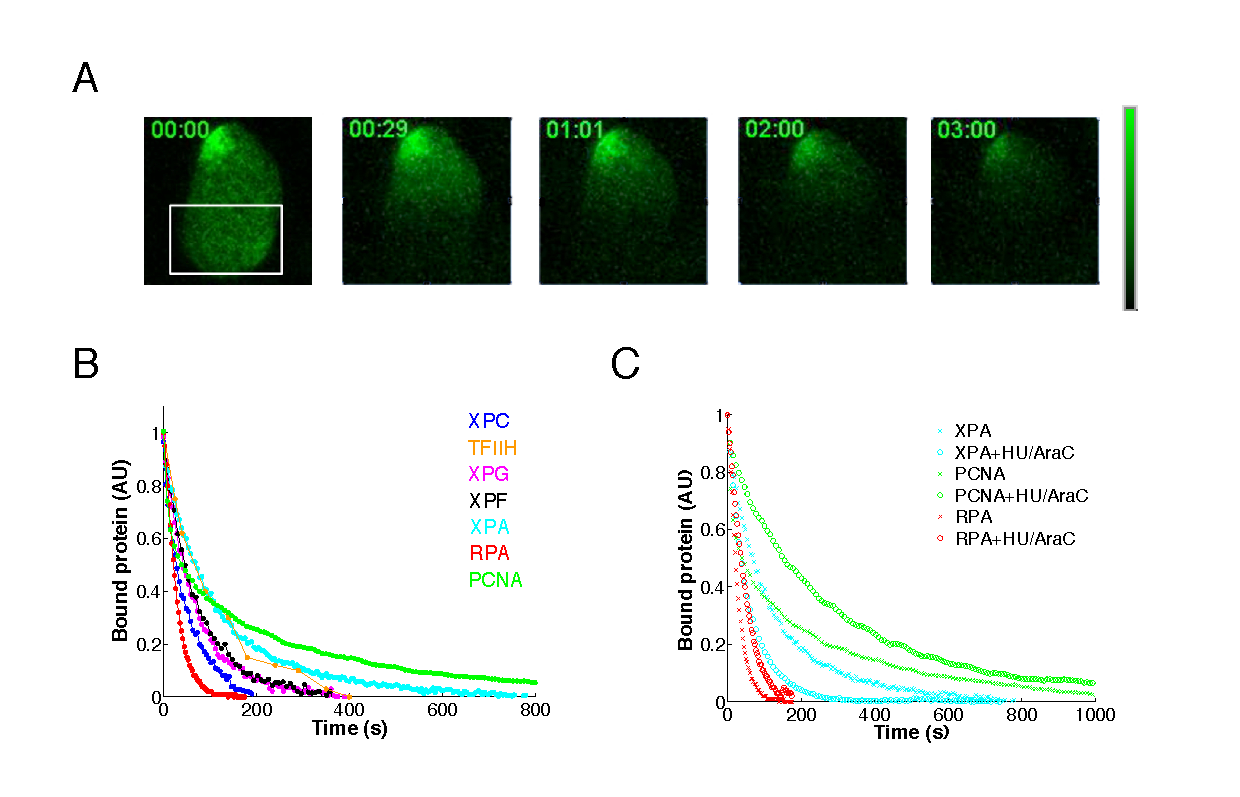
\includegraphics[width=1\textwidth]{Abbildungen/figure2_2_2.pdf}
  		\caption{\textbf{Rapid dissociation of NER factors from damaged DNA.} A) FLIP experiment in XP2OS cells stably expressing eGFP-XPA after 2 h of local irradiation. The nucleus is continuously bleached in an undamaged region (white rectangle). Fluorescence loss is recorded at the sites of local UV-irradiation B)\,Amount of bound NER-factors (XPC-eGFP, TFIIH-eGFP, XPG-eGFP, XPF-GFP, eGFP-XPA, RPA-eGFP and eGFP-PCNA) monitored over time at LD. C) Quantification of FLIP experiments in the absence or presence of HU and AraC for stably expressed eGFP-XPA, RPA-eGFP and eGFP-PCNA.}
  		\label{fig:accuFlip}
  	\end{center}
  \end{figure}



\section{Direct measurement of DNA resynthesis}
\label{Subsec:EdUmeasurement}

In order to expand our quantitative inspection of the NER pathway in intact mammalian cells, we established a protocol for the direct measurement of the repair synthesis process \cite{Verbruggen2014}. DNA resynthesis reflects the kinetics of the post-incision repair process, complementing the measurement of DNA lesion removal, which captures the system's behaviour of the pre-incision steps (cf.\ section \ref{sec:NERexperiments}). To mark newly-incorporated DNA shortly before and after local UV irradiation, cells were incubated in microscopy medium supplemented with 10 \textmu M 5-ethynyl-2'-deoxyuridine (EdU). Due to its excessive presence in solution, the DNA polymerase integrates EdU (a thymidine analogue) instead of the endogenous thymine into the new DNA strand (cf.\ Figure \ref{fig:EdU_measurement}A). After incubation for the desired time, cells were fixed, stopping EdU incorporation, and subsequently permeabilized. EdU was then tagged with the fluorescent azide (AlexaFluor-555, Life Technologies) forming a covalent bond by click chemistry \cite{Limsirichaikul2009}. Analogous to the quantification of NER factor dynamics, EdU intensities were captured with a laser scanning microscope (Zeiss).\\
\begin{figure}[b!]
	\begin{center}
		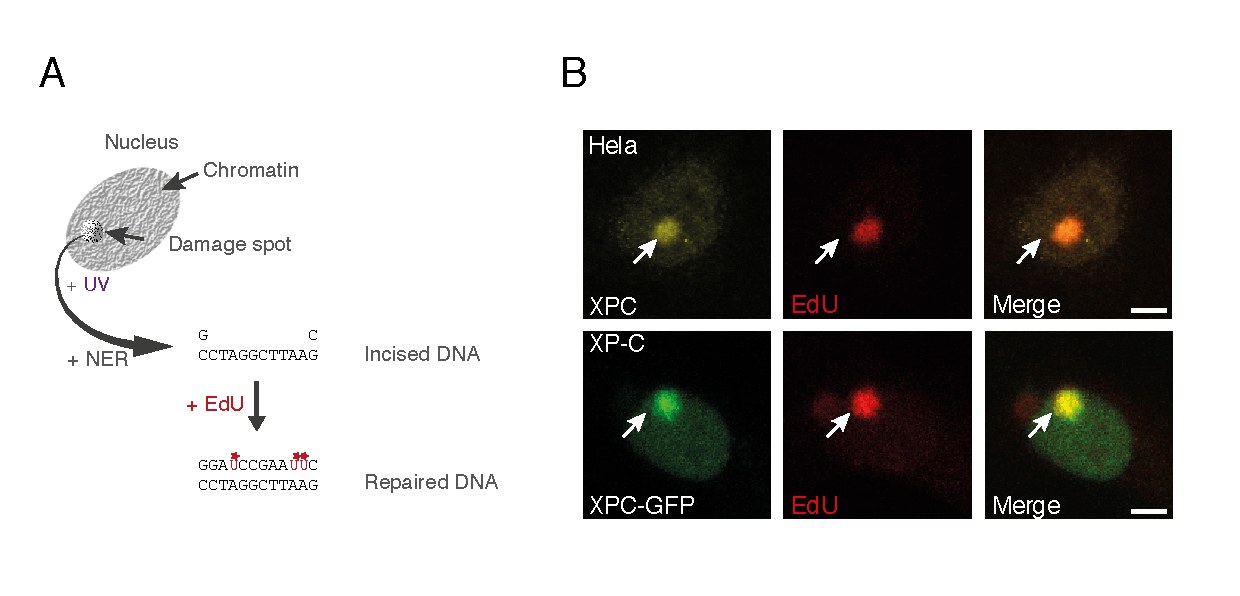
\includegraphics[width=1\textwidth]{Abbildungen/figure2_3.pdf}
		\caption{\textbf{EdU is incorporated at sites of local DNA damage.} A) Schematic illustration depicting the experimental procedure of EdU incorporation at sites of local damage. B) Antibody-stained endogenous XPC in Hela cells (upper panel) or stably expressed XPC-eGFP in XP-C cells (lower panel) accumulate in the LD spot and co-localize with incorporated EdU.}
		\label{fig:EdU_measurement}
	\end{center}
\end{figure}
\noindent Accordingly, incorporated EdU is exclusively present at the locally confined area of damaged and thereupon resynthesized DNA, which coincides with the localization of immunostained XPC (cf.\ Figure \ref{fig:EdU_measurement}B, upper row). The same result occurs for XP-C cells with stably-transfected XPC-eGFP (cf.\ Figure \ref{fig:EdU_measurement}B, lower row). Replicating cells could be excluded from the analysis due to the prevalent EdU incorporation distributed over the entire nucleus. 
  

    
 





\section{Repair rate follows first order rate kinetics}
\label{firstOrderRateKinetic}
In contrast to the real-time measurements for accumulation and dissociation of the NER factors, the incorporation of EdU cannot be followed continuously. As mentioned in section \ref{Subsec:EdUmeasurement}, cells have to be fixed and permeabilized before the newly incorporated bases can be fluorescently labelled. Therefore, only the accumulated EdU incorporated in the time interval between UV-irradiation and fixation can be followed. By repeating this procedure for growing time intervals we acquired successively the repair kinetics for newly-repaired DNA (cf.\ Figure \ref{fig:DNArepairKinetic}A and B). The signal at each time point represents the EdU signal averaged over multiple cells. \\
We found that EdU incorporation essentially stops after 4 hours, which coincides with the removal of 6-4PP (cf.\ \cite{Luijsterburg2010} and Figure \ref{fig:DNArepairKinetic}B). This agrees with the observation that NER is not primarily engaged in the removal of cyclobutane pyrimidine dimers (CPD) which are repaired on a much longer time scale \cite{Luijsterburg2010}. To test whether the availability of EdU is rate limiting, we measured the incorporation of EdU in discrete equidistant time intervals after UV-irradiation (cf.\ Figure \ref{fig:DNArepairKinetic}C). We observed that the amount of EdU incorporation per time interval (EdU rate) is indeed continuously declining and hence, the rate of repair synthesis. Moreover the EdU kinetic follows the trajectory of PCNA accumulation as measured by Luijsterburg \textit{et al.} \cite{Luijsterburg2010} (cf.\ Figure \ref{fig:DNArepairKinetic}D). PCNA is thought to act as processivity factor for the DNA polymerase and remains bound to the DNA \cite{Luijsterburg2010,Essers2005,Sporbert2002}. Taken together, these data establish EdU incorporation as a direct and quantitative measure for DNA repair synthesis in locally damaged nuclei.\\
The DNA repair time series characterized by incorporated EdU is fitted by a mono-exponential kinetic (cf.\ Figure \ref{fig:DNArepairKinetic}E):
\begin{equation}
EdU(t) = EdU_\text{max}(1 - e^{\lambda t}),
\label{Eqn:EdU_kinetic}
\end{equation}  
where $EdU(t)$ and $EdU_{\text{max}}$ give the amount of incorporated EdU and its value at saturation, respectively. The time constant was determined as $\lambda$=0.58 ($\pm$0.07) $\text{h}^{-\text{1}}$ using the polyfit function (pre-implemented in MATLAB). This result indicates that despite its molecular complexity, 6-4PP removal by NER is a slow first-order reaction with a half-time of 1.2 hours. \\
        
\begin{figure}[b!]
\begin{center}
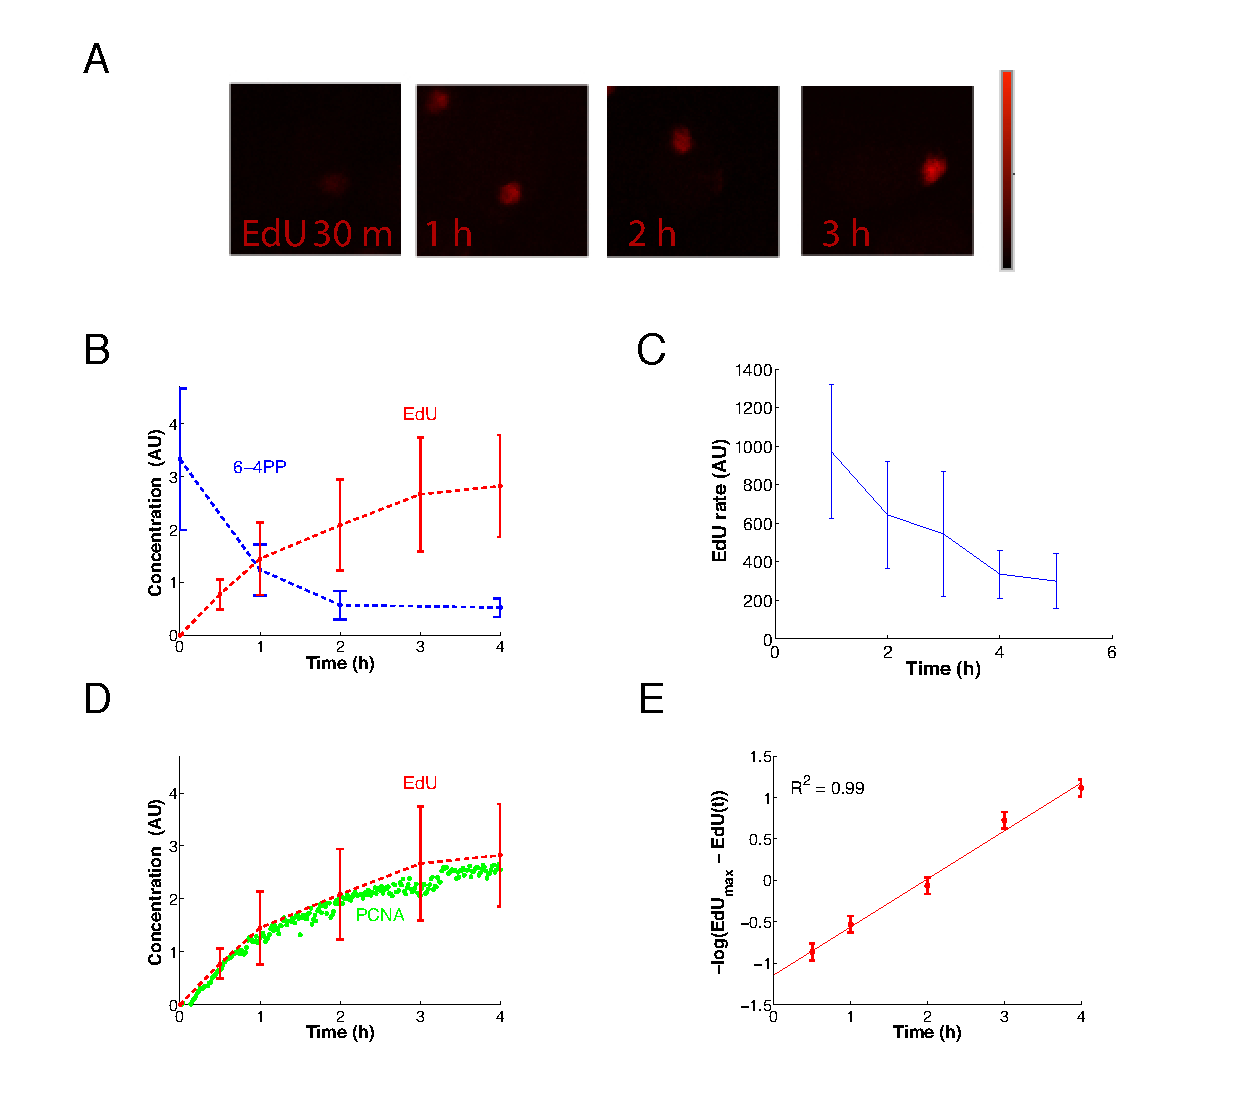
\includegraphics[width=1\textwidth]{Abbildungen/figure2_4.pdf}
\caption{\textbf{EdU incorporation reflects DNA repair synthesis quantitatively.} A) EdU signal at various time points after local UV-C irradiation. B) Repair DNA synthesis (EdU, red curve) coincides with damage removal (6-4PP, blue curve) measured previously by Luijsterburg \textit{et al.} (2010) \cite{Luijsterburg2010}. The EdU trajectory represents mean $\pm$\,SD (derived from three independent experiments) of DNA repair in locally damaged cells (n=150) per time point. C) Irradiated XP-C XPC-eGFP cells were treated with EdU for different time intervals post-irradiation. Intervals were chosen as follows: 15 minutes pre-irradiation to 60 minutes post-irradiation, 45-120 minutes, 105-180 minutes, 165-240 minutes and 225-300 minutes. Line plot represents mean $\pm$\,SD of EdU distributions derived from a particular time interval. D) DNA repair synthesis follows PCNA accumulation as measured previously \cite{Luijsterburg2010}. E) Mono-exponential fit of the EdU kinetic according to Eqn.\ \ref{Eqn:EdU_kinetic}.}
\label{fig:DNArepairKinetic}
% * <l.adlung@dkfz.de> 2014-12-07T10:08:06.916Z:
%
%  Explain UV-C in contrast to UV. Give R^2 for E
%
\end{center}
\end{figure}
Taken together, our experimental insight of the NER process got extended by following the kinetics of a repair intermediate directly. Now we are able to integrate our knowledge about the dynamic behaviour of individual repair factors and study its association with the overall repair rate quantitatively.    